\documentclass[12pt]{article}
\usepackage{graphicx}
\usepackage{xcolor}
\usepackage{geometry}
\geometry{margin=1in}

\begin{document}

\begin{center}

\includegraphics[width=0.3\textwidth]{iiitb_comet_logo.jpg}
\end{center}

\vspace{0.5cm}

\begin{center}
{\Large \textbf{Anushree M R}} \\
ID: COMETFWC063
\end{center}

\vspace{0.8cm}

\begin{center}
{\Large \textcolor{blue}{\textbf{GATE Question}}}
\end{center}

{\color{blue}\section*{Question:42}}

The logic gate circuit shown in the adjoining figure realizes the function.

\begin{center}
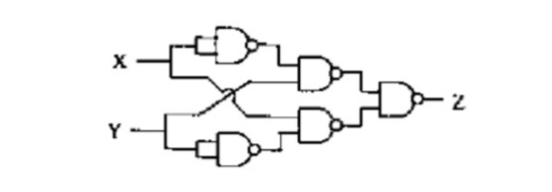
\includegraphics[width=0.75\textwidth]{gate_q41.jpg}
\end{center}

\textbf{Options}

\begin{itemize}
\item (a) XOR
\item (b) XNOR
\item (c) Half Adder
\item (d) Full Adder
\end{itemize}

{\color{blue}\section*{Question Analysis}}

From the circuit we observe that the logic gates combine the inputs X and Y in such a way that the output becomes HIGH when the inputs are different and LOW when they are the same.

This corresponds to the XOR operation.

\[
Z = X \oplus Y
\]

{\color{blue}\section*{Truth Table}}

\begin{center}
\begin{tabular}{|c|c|c|}
\hline
X & Y & Z \\
\hline
0 & 0 & 0 \\
0 & 1 & 1 \\
1 & 0 & 1 \\
1 & 1 & 0 \\
\hline
\end{tabular}
\end{center}

Hence the circuit represents the XOR function.

Correct Answer: \textbf{(a) XOR}

{\color{blue}\section*{Components Used}}

\begin{itemize}
\item Arduino UNO
\item IC 7447 (BCD to 7-segment decoder)
\item Common Anode 7-segment display
\item Breadboard
\item Jumper wires
\end{itemize}

{\color{blue}\section*{Pin Connections}}

Arduino Pin 10 $\rightarrow$ Input X

Arduino Pin 11 $\rightarrow$ Input Y

IC 7447 Pin 16 $\rightarrow$ 5V

IC 7447 Pin 8 $\rightarrow$ GND

7447 output pins connected to the segments of the 7-segment display through resistors.

Common anode of the display connected to 5V.

{\color{blue}\section*{Hardware Implementation}}

The inputs X and Y are given from Arduino UNO.  
The Arduino reads these inputs and performs the XOR logic operation.

If the output of the XOR operation is HIGH, the corresponding BCD signal is given to the IC 7447 decoder.

The IC 7447 then activates the required segments of the 7-segment display to show the output value.

Thus the circuit verifies the XOR logic function using hardware components.

{\color{blue}\section*{Conclusion}}

The given logic gate circuit implements the XOR operation.

\[
Z = X \oplus Y
\]

Hence the correct answer is:

\textbf{(a) XOR}

\end{document}
